

\documentclass{beamer}
 
\usepackage[utf8]{inputenc}
 
\setbeamertemplate{footline}[frame number]
\beamertemplatenavigationsymbolsempty
 
 
 
\usetheme{Madrid} 
 
\AtBeginSection[]{
  \begin{frame}
  \vfill
  \centering
  \begin{beamercolorbox}[sep=8pt,center,shadow=true,rounded=true]{title}
    \usebeamerfont{title}\insertsectionhead\par%
  \end{beamercolorbox}
  \vfill
  \end{frame}
} 
 
 
 
 
 
 
 
\theoremstyle{plain}
\newtheorem{thm}{Theorem}[section] % reset theorem numbering for each chapter

\theoremstyle{definition}
\newtheorem{defn}[thm]{Definition} % definition numbers are dependent on theorem numbers
\newtheorem{exmp}[thm]{Example} % same for example numbers

%Information to be included in the title page:
\title{Causality in Multi-Agent Planning}
\author{Axel Ind}
\institute{ALU-Freiburg}
\date{\today}
 
 
 
\begin{document}
 
\frame{\titlepage}

\section{Halpern's Causality}

\begin{frame}
\frametitle{Alice}
\begin{itemize}
\item This is Alice.
\item Alice is studying.
\item But she's not a very good student.
\end{itemize}

\begin{figure}
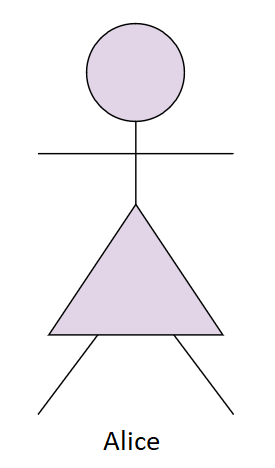
\includegraphics[scale=0.5]{alice}
\end{figure}

\end{frame}



\begin{frame}
\frametitle{Alice}
\begin{itemize}
\item Alice did not hand in any homework.
\item Alice failed her class.
\item Why did Alice fail?
\end{itemize}

\begin{figure}
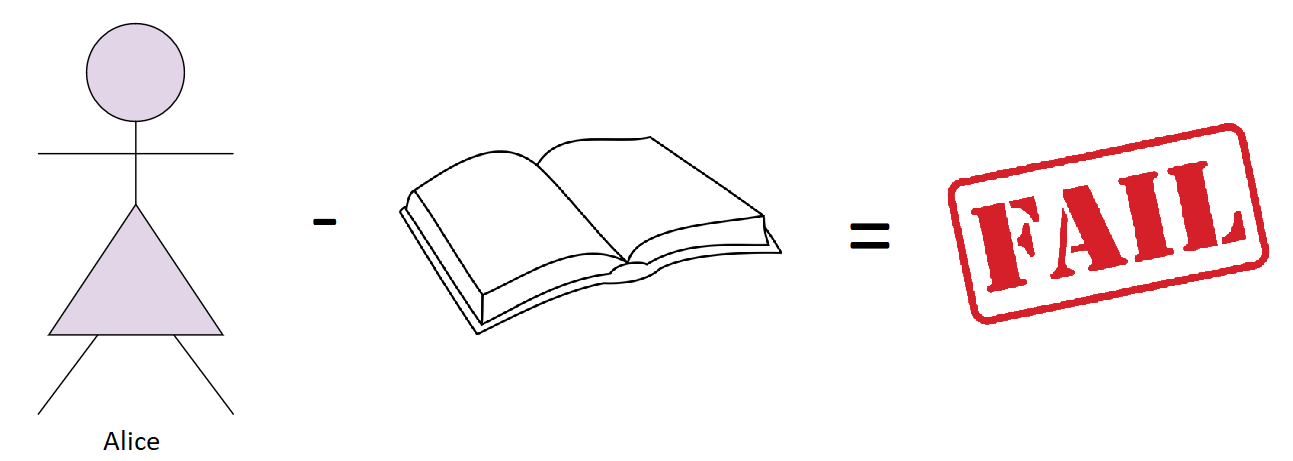
\includegraphics[scale=0.3]{aliceFail}
\end{figure}

\end{frame}


\begin{frame}
\frametitle{Bob}
\begin{itemize}
\item This is Bob.
\item Bob likes fires.
\item ... A little too much.
\item Bob is an arsonist.
\item And he has found a box of matches.
\end{itemize}

\begin{figure}
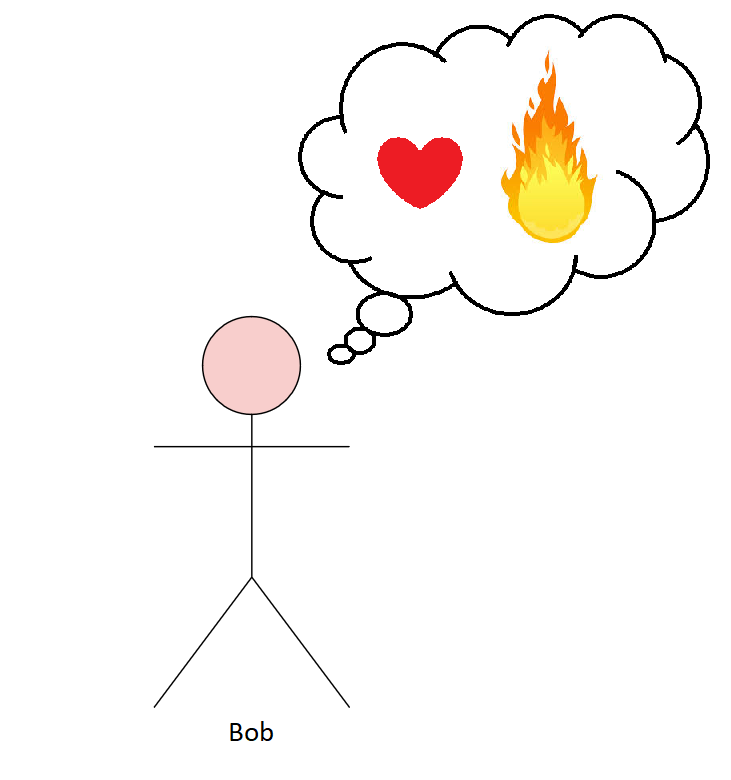
\includegraphics[scale=0.23]{bobFire}
\end{figure}
\end{frame}


\begin{frame}
\frametitle{Bob}
\begin{itemize}
\item Bob is in a forest.
\item He drops a lit match.
\item At the same moment, lightning strikes.
\item The forest burns down.
\item Why did the forest burn down?
\end{itemize}

\begin{figure}
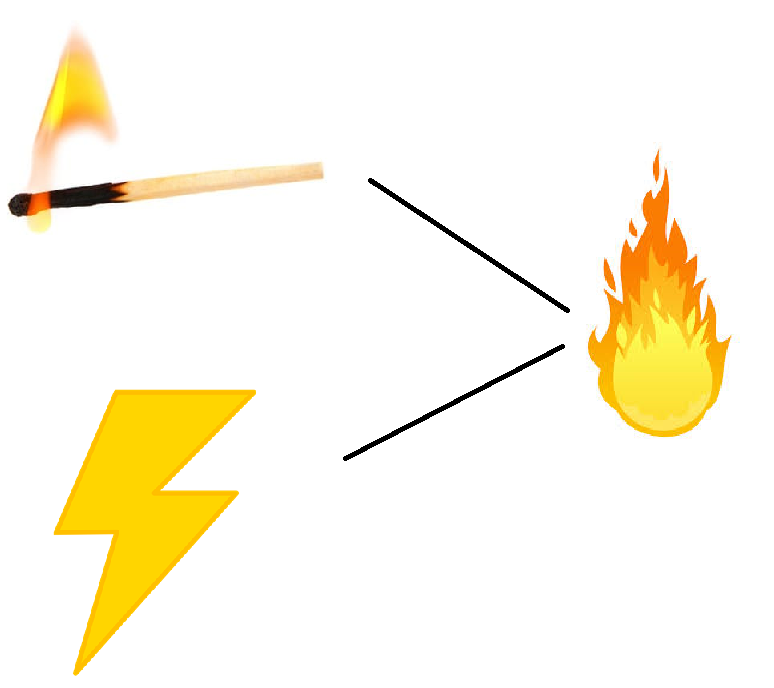
\includegraphics[scale=0.25]{bobLightningFire}
\end{figure}
\end{frame}



\begin{frame}
\frametitle{Alice and Bob}
\begin{itemize}
\item Alice and Bob are friends.
\item They find an empty house.
\item They decide to throw stones at the windows.
\end{itemize}

\begin{figure}
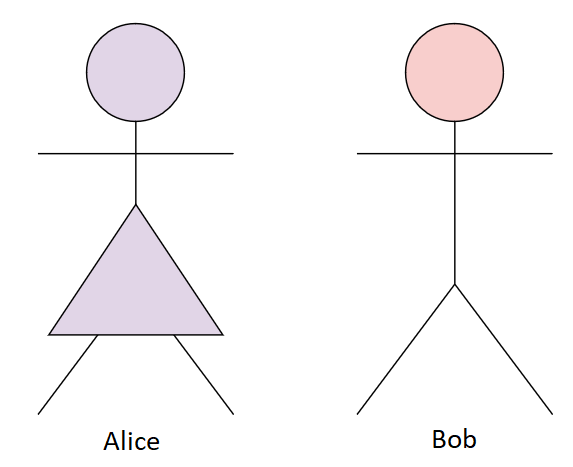
\includegraphics[scale=0.4]{aliceandbob}
\end{figure}

\end{frame}



\begin{frame}
\frametitle{Alice}
\begin{itemize}
\item They each throw a stone.
\item The window shatters.
\item Who should we blame?
\end{itemize}

\begin{figure}
\includegraphics[scale=0.15]{stoneWindow}
\end{figure}

\end{frame}


\begin{frame}
\frametitle{A Brief Overview}
\begin{itemize}
\item What is causality?
\item Halpern's Causality.
\item Counterfactaul reasoning in planning.
\item Planning Causality.
\end{itemize}

\end{frame}
%=========================================================================
%=========================================================================
%=========================================================================





\begin{frame}
\frametitle{My Contributions}
\begin{itemize}
\item Multi-agent framework for causality.
\item Four types of causality in planning.
\end{itemize}

\begin{figure}
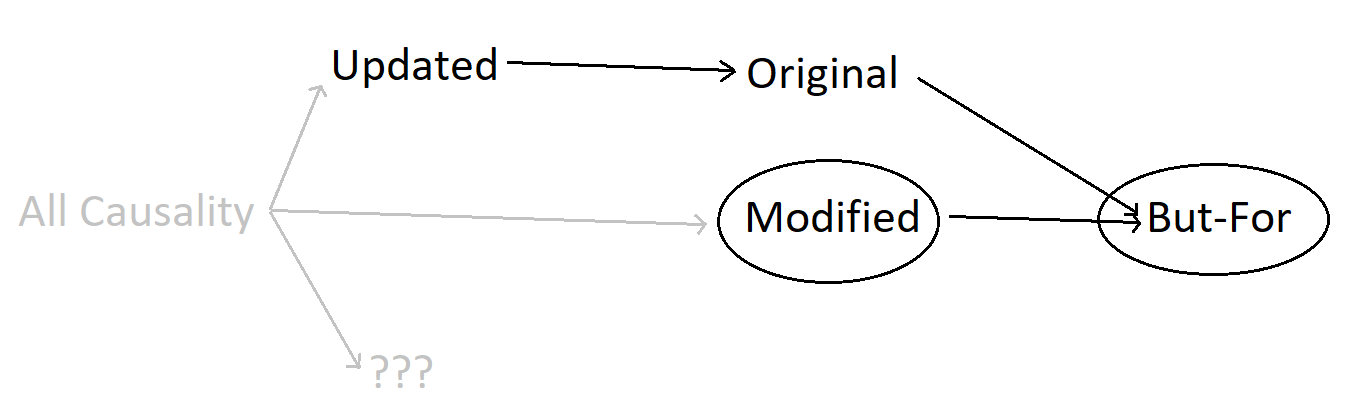
\includegraphics[scale=0.35]{causaldiagram}
\end{figure}
\end{frame}


 
\begin{frame}
\frametitle{What is Causality?}
\begin{itemize}
\item $A$ caused $B$.
\item Our intuitions differ.
\item @TODO ref formalised their own definitions.

\end{itemize}

\end{frame}

\begin{frame}
\frametitle{Alice's Homework}
\begin{itemize}
\item ``If Alice had not done her homework, she would have failed."
\item Possible cause: not doing her homework.
\item What if she \textit{had} done it?
\end{itemize}

\begin{figure}
\includegraphics[scale=0.31]{alicepass}
\end{figure}

\end{frame}



%========================================HP CAUSALITY===============================

\section{Halpern's Causality}


\begin{frame}
\frametitle{Halpern's Causality}

\begin{itemize}
\item The causal setting.
\item Allows counter-factual reasoning.
\item Unambiguous causality in this framework.

\end{itemize}

\end{frame}

\begin{frame}
\frametitle{Causal Settings: Alice's Homework}
\begin{itemize}
\item Causal setting $(M,u)$.
\item Sufficient to the initial and final state of the world.

\end{itemize}

\begin{figure}
\includegraphics[scale=0.3]{alicemodel}
\end{figure}
\end{frame}

\begin{frame}
\frametitle{Causal Settings: Bob's Fire}
\begin{figure}
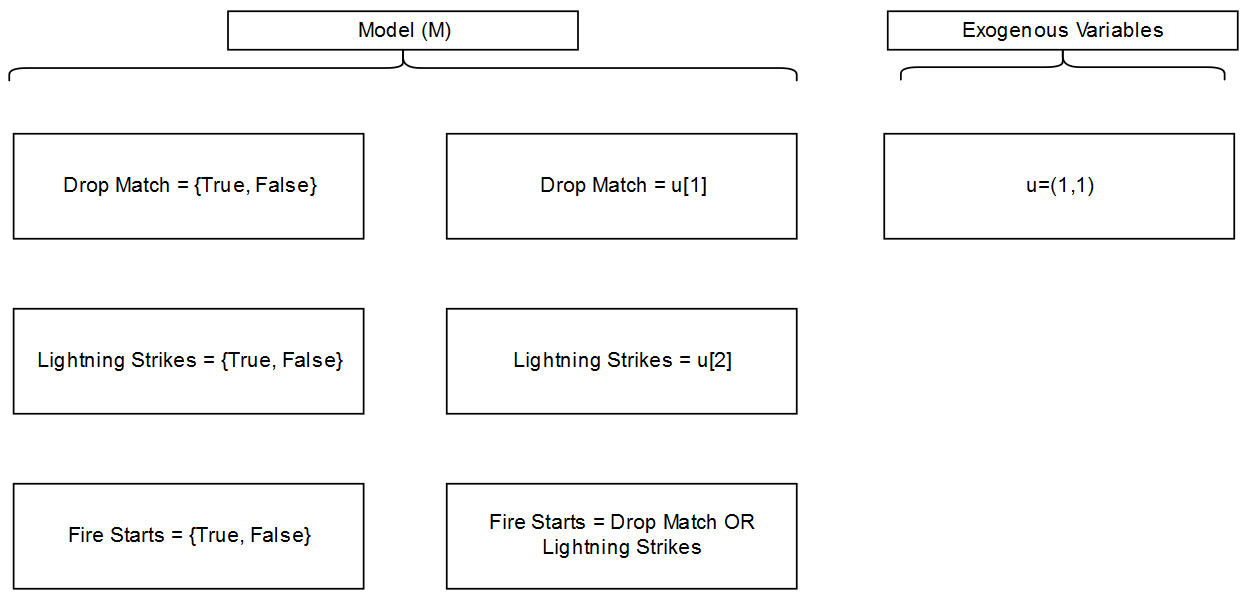
\includegraphics[scale=0.3]{fireModel}
\end{figure}
\end{frame}


\begin{frame}
\frametitle{Causal Settings: Alice and Bob}
\begin{figure}
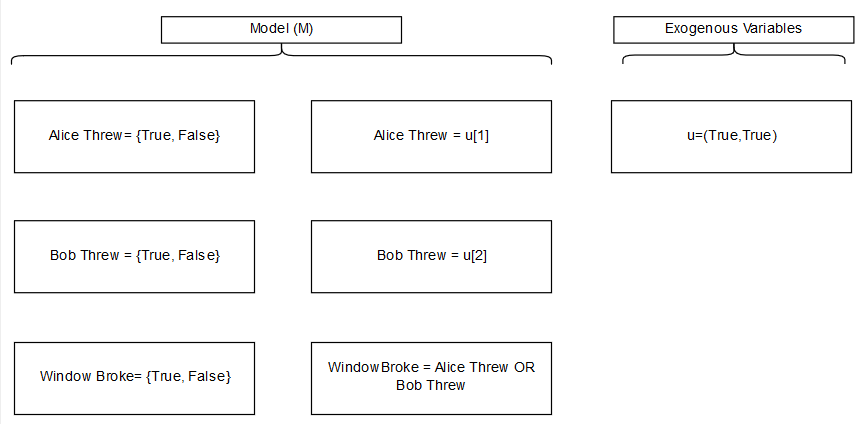
\includegraphics[scale=0.4]{aliceBobModel1}
\end{figure}
\begin{itemize}
\item Identical to the Forest Fire example.
\item How can we change it?
\end{itemize}
\end{frame}

\begin{frame}
\frametitle{Causal Settings: Alice and Bob}
\begin{figure}
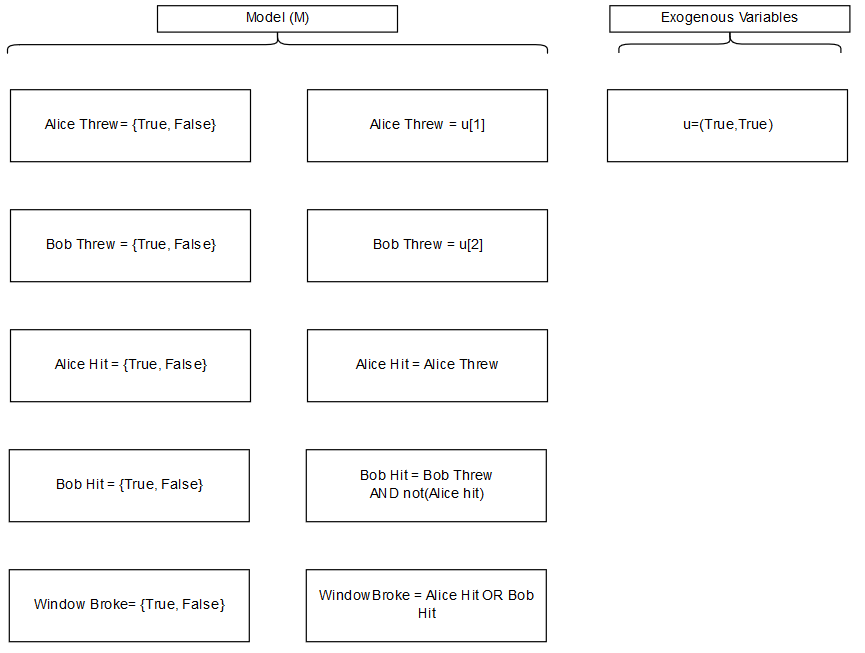
\includegraphics[scale=0.4]{aliceBobModel2}
\end{figure}
\end{frame}



\begin{frame}
\frametitle{But-For Causality}
\begin{itemize}
\item ``$X=x$ is a cause of $\phi$" if changing the value of $X$ to $x'$ means that $\phi$ no longer holds.
\end{itemize}
\end{frame}



\begin{frame}
\frametitle{But-For Causality}

\begin{defn}$X=x$ is a but-for cause of $\phi$ in the causal setting $(M,u)$ iff the following 3 conditions hold:
\begin{enumerate}
\item $(M,u) \models (X=x)$ and $(M,u) \models \phi$.
\item $AC2(bf)$: There is a setting $x'$ of the variables in $X$ such that

\[
(M,u) \models [X\leftarrow x']\lnot \phi
\] 

\item $X$ is minimal, there is no strict subset $X'$ of $X$ such that $X' = x'$ satisfies the above conditions.
\end{enumerate}

\end{defn}

\end{frame}


\begin{frame}
\frametitle{Example 1: Alice's Homework}

\begin{itemize}
\item In the actual world she didn't do her homework and failed.
\end{itemize}
\begin{figure}
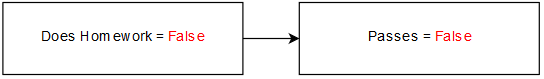
\includegraphics[scale=.4]{aliceModelReal}
\end{figure}


\begin{itemize}
\item In our model, counter-factually examining the world in which she did her homework results in her passing.
\end{itemize}
\begin{figure}
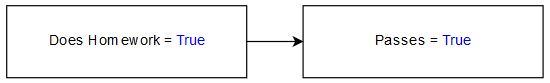
\includegraphics[scale=.4]{aliceModelCounterfactual}
\end{figure}

\end{frame}


\begin{frame}
\frametitle{Example 2: Bob's Fire}
\begin{figure}
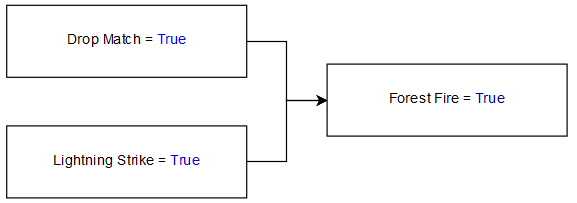
\includegraphics[scale=.4]{bobModelReal}
\end{figure}

\begin{itemize}
\item Counter-factually stating that Bob did not drop the match still results in the forest fire.
\end{itemize}
\begin{figure}
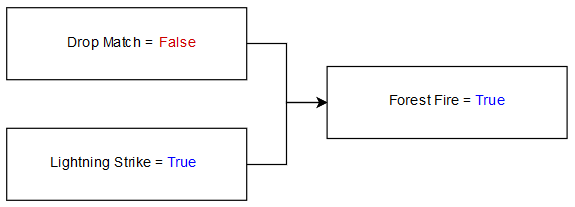
\includegraphics[scale=.4]{bobModelCounterfactual}
\end{figure}

\end{frame}


\begin{frame}
\frametitle{Example 2: Bob's Fire}

\begin{itemize}
\item If neither the match was dropped nor the lightning struck, there would have been no forest fire.
\end{itemize}
\begin{figure}
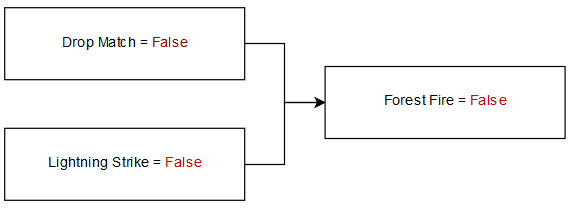
\includegraphics[scale=.4]{bobModelCounterfactual2}
\end{figure}

\begin{itemize}
\item $X = \{Drop Match = True\}$ is not a cause of $forest fire$, but $X = \{Drop Match = True, Lightning Strike = True\}$ is a cause.
\end{itemize}

\end{frame}


\begin{frame}
\frametitle{Example 3: Alice and Bob's Window}
\begin{figure}
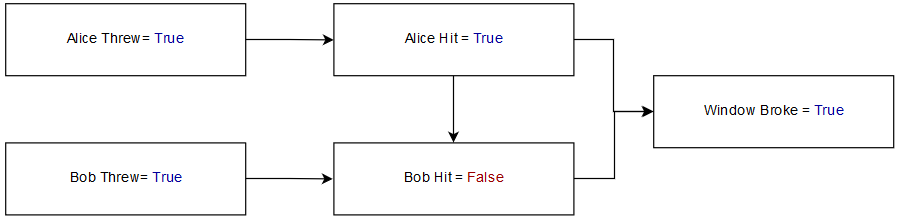
\includegraphics[scale=.4]{alicebobModelReal}
\end{figure}

\begin{itemize}
\item With $x' = \{ Alice Threw = False\}$, Bob's stone now breaks the window.
\end{itemize}
\begin{figure}
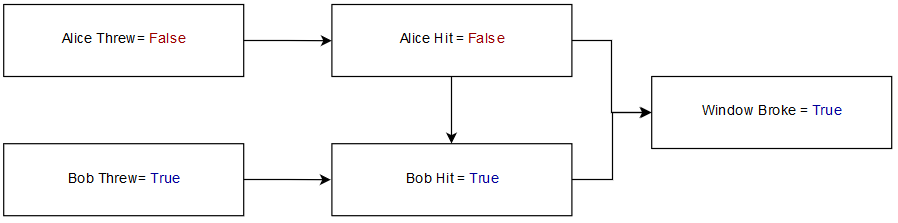
\includegraphics[scale=.4]{alicebobModelCounterfactual}
\end{figure}
\end{frame}

\begin{frame}
\frametitle{Example 3: Alice and Bob's Window}
\begin{figure}
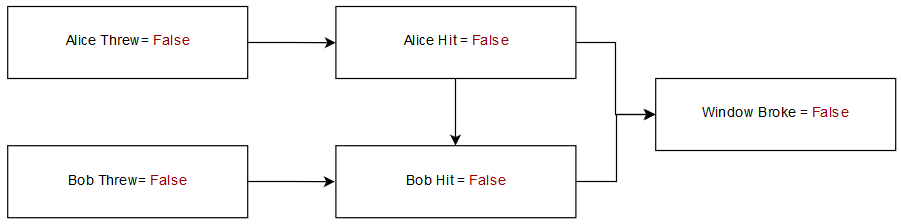
\includegraphics[scale=.4]{alicebobModelCounterfactual2}
\end{figure}

\begin{itemize}
\item $X = \{Alice Threw = True\}$ is not a cause of $Bottle Broke = True$.
\item $X = \{Alice Threw = True, Bob Threw = True\}$ is a cause of $Bottle Broke = True$.
\end{itemize}
\end{frame}



\begin{frame}
\frametitle{Halpern's Modified Causality}
\begin{itemize}
\item Intuitively we might feel that Alice is a cause, but Bob is not.
\item But-for causality is limited.
\item Extends but-for causality.
\end{itemize}

\end{frame}

\begin{frame}
\frametitle{Halpern's Modified Causality}
\begin{defn}$X=x$ is an actual cause of $\phi$ in the causal setting $(M,u)$ iff the following 3 conditions hold:
\begin{enumerate}
\item $(M,u) \models (X=x)$ and $(M,u) \models \phi$.
\item $AC2(a^m)$: There is a set $\vec{W}$ of variables in $V$ and a setting $x'$ of the variables in $X$ such that if $(M,u) \models W = w^*$, then:
\[
(M,u) \models [X \leftarrow x', W \leftarrow w^*] \neg \phi
\]
\item $X$ is minimal. There is no strict subset of $X$ that satisfies the previous 2 conditions.
\end{enumerate}

\end{defn}
\end{frame}

\begin{frame}
\frametitle{Example 1: Alice's Homework}

\begin{figure}
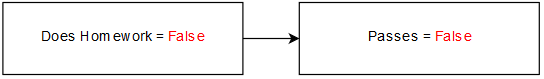
\includegraphics[scale=.5]{aliceModelReal}
\end{figure}

\begin{itemize}
\item A But-For cause is a cause in the Modified definition with $W=\{\}$.
\end{itemize}

\begin{figure}
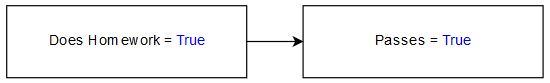
\includegraphics[scale=.5]{aliceModelCounterfactual}
\end{figure}

\begin{itemize}
\item $X=\{Does Homework = True\}$ is a cause in Modified Definition.
\end{itemize}


\end{frame}


\begin{frame}
\frametitle{Example 2: Bob's Fire}
\begin{figure}
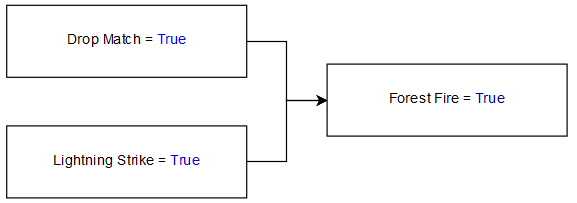
\includegraphics[scale=.5]{bobModelReal}
\end{figure}

\begin{figure}
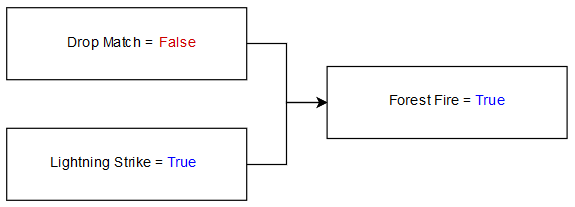
\includegraphics[scale=.5]{bobModelCounterfactual}
\end{figure}
\begin{itemize}
\item No matter what other variables we find as $W$, we can't cause $Forest Fire = False$.
\end{itemize}
\end{frame}

\begin{frame}
\frametitle{Example 2: Bob's Fire}
\begin{figure}
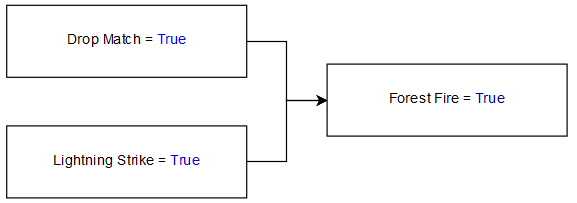
\includegraphics[scale=.5]{bobModelReal}
\end{figure}

\begin{figure}
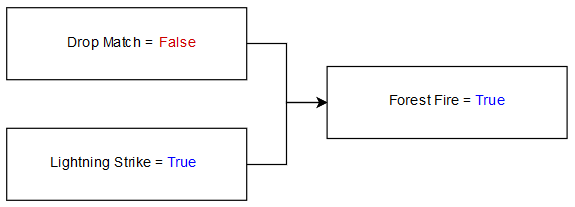
\includegraphics[scale=.5]{bobModelCounterfactual}
\end{figure}
\end{frame}

\begin{frame}
\frametitle{Example 2: Bob's Fire}
\begin{figure}
\includegraphics[scale=.5]{bobModelCounterFactual2}
\end{figure}

\begin{itemize}
\item $X=\{Drop Match=True, Lightning Strike = True\}$, with $W=\{\}$ is a cause of $Forest Fire = True$
\end{itemize}
\end{frame}


\begin{frame}
\frametitle{Example 3: Alice and Bob's Window}
\begin{figure}
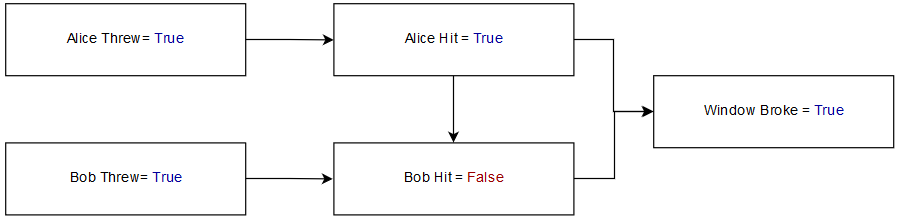
\includegraphics[scale=.40]{alicebobModelReal}
\end{figure}

\begin{figure}
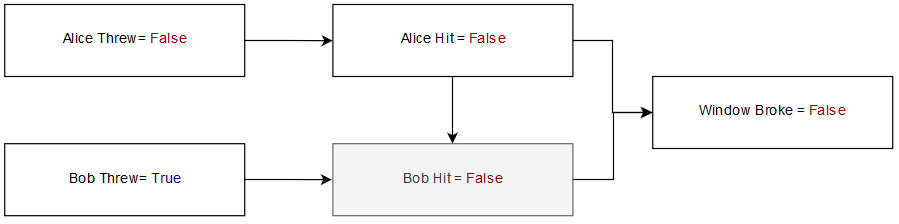
\includegraphics[scale=.40]{alicebobModelCounterfactual3}
\end{figure}

\begin{itemize}
\item By fixing $W=\{Bob Hit = True\}$, $X=\{Alice Threw = True\}$ is cause of $Window Broke = True$.
\end{itemize}
\end{frame}

\section{Causality in Planning}

\begin{frame}
\frametitle{Causality in Planning}
\begin{itemize}
\item Causal settings require independent structural equations.
\item Planning is more expressive.
\item Idea: extend HP's Causality for AI Planning.
\end{itemize}

\end{frame}



\begin{frame}
\frametitle{Why is Planning Causality Different?}
\begin{itemize}
\item Actions and variables are distinct.
\item Exogenous actions.
\item Sequential ordering of actions.
\item Identify agent causes.
\end{itemize}

\end{frame}


\begin{frame}
\frametitle{Single-Agent Planning Tasks}
\begin{figure}
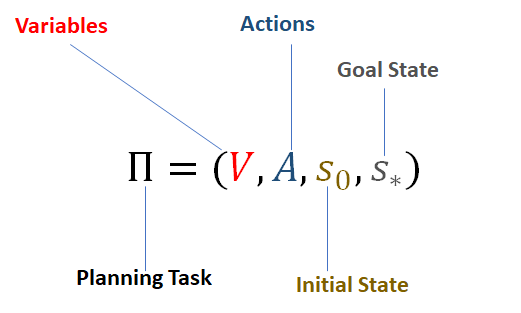
\includegraphics[scale=.5]{planningTask}
\end{figure}

\end{frame}


\begin{frame}
\frametitle{Exogenous Actions}
\begin{itemize}
\item Not performed by any agent.
\item Can be timed, or we get non-determinism.
\item Unlike @TODOref we allow conflicting exogenous actions.
\end{itemize}

\end{frame}


\begin{frame}
\frametitle{Plans}
\begin{itemize}
\item A plan $\pi$ is a sequence of actions. 

\item We define \textit{action slots}. 

\end{itemize}


\begin{defn}
An action slot $q(\pi,k)$ is mapped to the list of all applicable actions at position $k$ in the plan. Intuitively an action slot functions like a variable name for the domain of possible actions at a specific time-point in $\pi$.
\end{defn}

\end{frame}


\begin{frame}
\frametitle{CPS New Operations}
\begin{itemize}
\item A subplan $\pi'$, $\pi'\subset \pi$ is a subset of the action slots in $\pi$.
\item A plan and a subplan are not interchangeable.
\end{itemize}

\begin{figure}
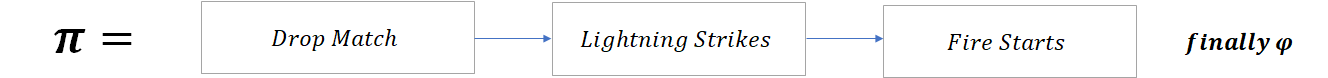
\includegraphics[scale=.30]{bobPlanOriginal}
\end{figure}
\begin{figure}
\includegraphics[scale=.35]{bobPlan}
\end{figure}

\begin{itemize}
\item Valid $\pi'$ values: $\{q(\pi',1),q(\pi',2),q(\pi',3)\}$, $\{q(\pi',1),q(\pi',2)\}$, $\{q(\pi',1),q(\pi',3)\}$, $\{q(\pi',2),q(\pi',3)\}$, $\{q(\pi',2),q(\pi',3)\}$, $\{(\pi',1)\}$,$\{(\pi',2)\}$, $\{(\pi',3)\}$
\end{itemize}

\end{frame}

\begin{frame}
\frametitle{Causal Plan Settings}
\begin{itemize}
\item We define the Casual Plan Setting $(\pi, \Pi)$.
\item Similar intuition to causal settings.
\newline
\end{itemize}


\[
(\pi,\Pi)\models (\textrm{finally} \phi)
\]

iff execution of the plan results in the variable assignments $\phi$ in the final state.

\[
(\Pi, \pi)[\pi'\leftarrow o'] \models (\textrm{finally} \phi)
\]
iff counterfactually using actions $o'$ in the CPS would result in $\phi$.

\end{frame}




\begin{frame}
\frametitle{But-For Causality Planning}
\begin{itemize}
\item ``Would changing $\pi'$ from $\pi'=o$ to $\pi'= o'$ change the final value of some variables $\phi$?"
\end{itemize}

\end{frame}

\begin{frame}
\frametitle{But-For Causality Planning}
\begin{defn} 

Given a planning task $\Pi$ and a plan $\pi$ with a final state $s_n$, some action slots in $\pi$, $\pi' \subseteq \pi$, $\pi' \leftarrow o$ are a But-For cause of some final variable assignment $s_n \models \phi$ iff the following 3 conditions hold:
\begin{enumerate}
\item  $o \subseteq \pi$, $\pi' \models o$ and $s_n \models \phi$.
\item $BF2$: There is a setting $o'$ of the non-$\epsilon$ action slots in $\pi'$ such that:
\[
(\pi, \Pi) \models [\pi' \leftarrow o'](\lnot \textrm{finally} \phi)
\]
\item $\pi'$ is minimal. There is no strict subset of $\pi'$ that satisfies the previous 2 conditions.
\end{enumerate}


\end{defn}

\end{frame}
\begin{frame}
\frametitle{Example 1: Alice's Homework}
\begin{figure}
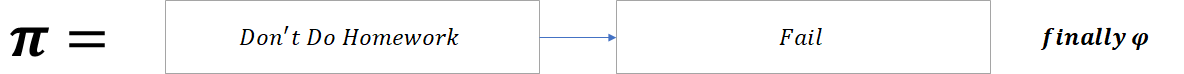
\includegraphics[scale=.35]{alicePlan}
\end{figure}

\begin{itemize}
\item What other actions could Alice have taken taken?
\item $\pi'= q(\pi,1)$, $o'=(Don't Do Homework)$
\end{itemize}

\begin{figure}
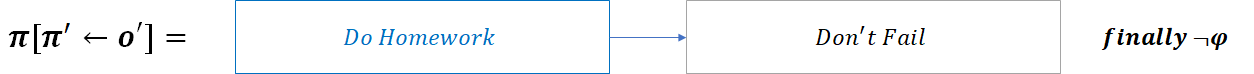
\includegraphics[scale=.35]{alicePlanCounterfactual}
\end{figure}
\end{frame}


\begin{frame}
\frametitle{Example 2: Bob's Fire}

\begin{figure}
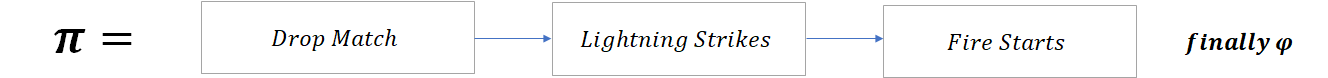
\includegraphics[scale=.33]{bobPlanOriginal}
\end{figure}
\begin{itemize}
\item $\pi'= q(\pi,1)$, $o'=\{Drop Match\}$
\end{itemize}
\begin{figure}
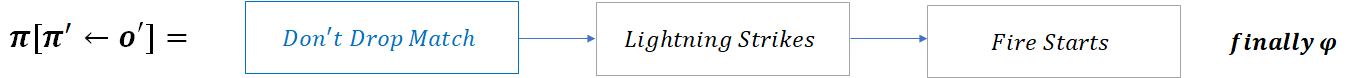
\includegraphics[scale=.32]{bobPlanCounterfactual}
\end{figure}

\begin{itemize}
\item $\pi'= \{q(\pi,1),q(\pi,2)\}$, $o'=\{Drop Match, Lightning Strikes\}$
\end{itemize}

\begin{figure}
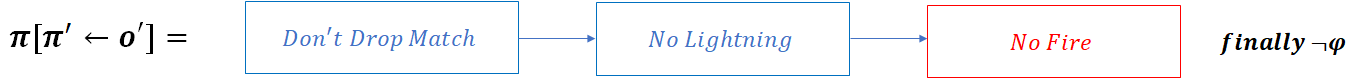
\includegraphics[scale=.32]{bobPlanCounterfactual2}
\end{figure}
\end{frame}


\begin{frame}
\frametitle{Example 3: Alice and Bob's Window}
\begin{figure}
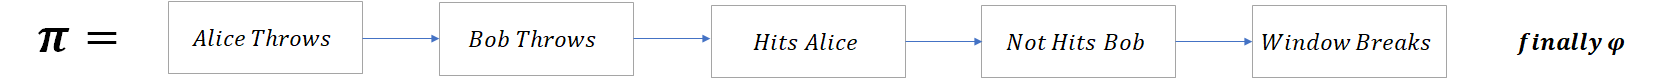
\includegraphics[scale=.28]{alicebobPlanOriginal}
\end{figure}
\begin{itemize}
\item $\pi'=\{q(1,\pi)\}$, $o'=\{Not Alice Throws\}$
\end{itemize}
\begin{figure}
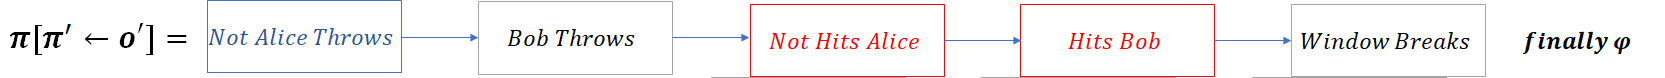
\includegraphics[scale=.28]{alicebobPlanCounterfactual}
\end{figure}
\begin{itemize}
\item $\pi'=\{q(1,\pi)\, q(2,\pi)\}$, $o'=\{Not Alice Throws, Not Bob Throws\}$
\end{itemize}
\begin{figure}
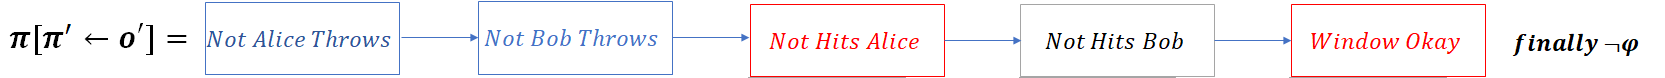
\includegraphics[scale=.28]{alicebobPlanCounterfactual2}
\end{figure}
\end{frame}

\begin{frame}
\frametitle{Modified Causality Planning}
\begin{defn}
Given a planning task $\Pi$ and plan $\pi$ with a final state $s_n$, some action slots $\pi'$,$\pi' \subseteq \pi$, $\pi' \leftarrow o$ are a cause of some final variable assignment $s_n \models \phi$ according to the modified planning definition iff the following 3 conditions hold:
\begin{enumerate}
\item  $o \subseteq \pi$, $\pi' \models o$ and $s_n \models \phi$.
\item $BF2$: There is a setting $o'$ of the applicable actions in $\pi'$, and a setting of $W \subseteq (\pi  - \pi')$ such that:
\[
(\pi, \Pi) \models [\pi' \leftarrow o', W \leftarrow w^\star](\lnot \textrm{finally}\phi)
\]
\item $\pi'$ is minimal. There is no strict subset of $\pi'$ that satisfies the previous 2 conditions.
\end{enumerate}


\end{defn}

\end{frame}

\begin{frame}
\frametitle{Example 1: Alice's Homework}
\begin{figure}
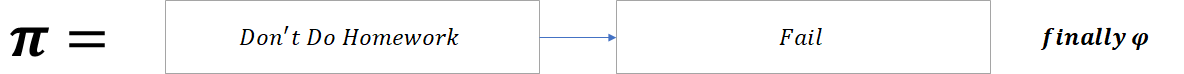
\includegraphics[scale=.35]{alicePlan}
\end{figure}

\begin{itemize}
\item $\pi'= q(\pi,1)$, $o'=(Don't Do Homework), W=\{\}$
\end{itemize}

\begin{figure}
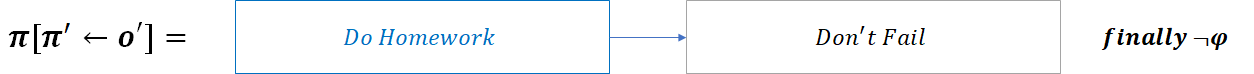
\includegraphics[scale=.35]{alicePlanCounterfactual}
\end{figure}
\end{frame}


\begin{frame}
\frametitle{Example 2: Bob's Fire}

\begin{figure}
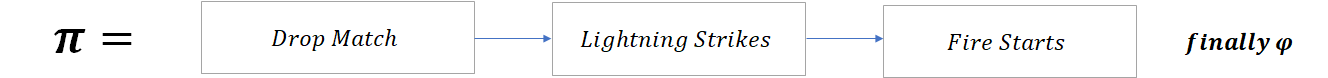
\includegraphics[scale=.28]{bobPlanOriginal}
\end{figure}

\begin{itemize}
\item $\pi'=\{ q(\pi,1)\}, o'=\{Don't Drop Match\}, W=\{\}$
\end{itemize}
\begin{figure}
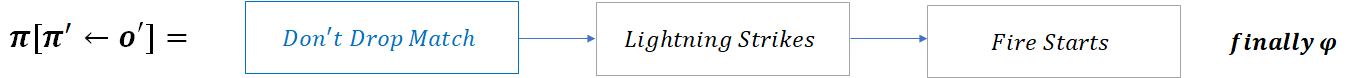
\includegraphics[scale=.28]{bobPlanCounterfactual}
\end{figure}

\begin{itemize}
\item $\pi'=\{q(1,\pi)\, q(2,\pi)\}$, $o'=\{Not Alice Throws, Not Bob Throws\}, W=\{\}$
\end{itemize}
\begin{figure}
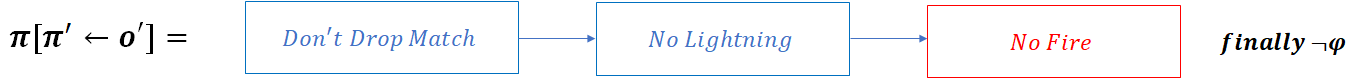
\includegraphics[scale=.28]{bobPlanCounterfactual2}
\end{figure}

\end{frame}


\begin{frame}
\frametitle{Example 3: Alice and Bob's Window}

\begin{figure}
\includegraphics[scale=.28]{aliceBobPlanOriginal}
\end{figure}

\begin{itemize}
\item $\{q(\pi,1) \}$, $o'=\{Not Alice Throws\}$, $W=\{q(\pi, 3\}$, $w^\star=\{ Not Hits Bob\}$
\end{itemize}
\begin{figure}
\includegraphics[scale=.28]{aliceBobPlanCounterfactual3}
\end{figure}
\end{frame}


\begin{frame}
\frametitle{Conclusions}
\begin{itemize}
\item @TODO ref's causality.
\item Extending Causality.
\item Future Work.
\end{itemize}

\end{frame}

\begin{frame}
\frametitle{Special Thanks}

\end{frame}


























\begin{frame}
\frametitle{Halpern's Original Causality}
\begin{itemize}
\item But-for causality catches only very simple intuitive causality.
\item Halpern introduce his Original Causality to account for this deficiency.
\item It asks two questions:
\begin{enumerate}
\item Is there any setting of the variables in the model such that $\phi$ no longer holds.
\item Is there any setting of variables in the model such that $X=x$ would be a but-for cause of $\phi$.
\end{enumerate}
\end{itemize}

\end{frame}


\begin{frame}
\frametitle{Halpern's Original Causality}
\begin{defn}$X=x$ is an actual cause of $\phi$ in the causal setting $(M,u)$ according to the original causality definition iff:
\begin{enumerate}
\item $(M,u) \models (X=x)$ and $(M,u) \models \phi$.
\item $AC2(a)$: There is a partition of $V$ (the endogenous variables) into two disjoint subsets $Z$ and $W$ with $X'\subseteq Z'$ and a setting $x'$ and $w$ of the variables in $X$ and $W$, respectively, such that

\[
(M,u) \models [X\leftarrow x', W\leftarrow w]\lnot \phi
\] 

\item $AC2(b^o)$: If $z^\star$ is such that $(M,u)\models Z = z^\star$, then for all subsets $Z'$ of $Z-X$, we have

\[
(M,u) \models [X\leftarrow x, W \leftarrow w, Z' \leftarrow z^\star]\phi
\] 

\item $X$ is minimal, there is no strict subset of $X'$ of $X$ such that $X' = x'$ satisfies the above conditions.
\end{enumerate}

\end{defn}
\end{frame}




\begin{frame}
\frametitle{Halpern's Updated Causality}
\begin{itemize}


\item Eventually Halpern found cases in which even his Original definition of causality did not seem to capture human intuition (e.g. the voting scenario which we will discuss later.)
\item He introduced his updated version of causality to ensure that the Original Causality definition held for every possible subset of $W$, $W'$.
\end{itemize}
\end{frame}


\begin{frame}
\frametitle{Halpern's Updated Causality}
\begin{defn}$X=x$ is an actual cause of $\phi$ in the causal setting $(M,u)$ according to the updated causality definition iff:
\begin{enumerate}
\item $(M,u) \models (X=x)$ and $(M,u) \models \phi$.
\item $AC2(a)$: There is a partition of $V$ (the endogenous variables) into two disjoint subsets $Z$ and $W$ with $X'\subseteq Z'$ and a setting $x'$ and $w$ of the variables in $X$ and $W$, respectively, such that

\[
(M,u) \models [X\leftarrow x', W\leftarrow w]\lnot \phi
\] 

\item $AC2(b^u)$: If $z^\star$ is such that $(M,u)\models Z = z^\star$, then for all subsets $Z'$ of $Z-X$ and $W'$ of $W$, we have

\[
(M,u) \models [X\leftarrow x, W' \leftarrow w, Z' \leftarrow z^\star]\phi
\] 

\item $X$ is minimal, there is no strict subset of $X'$ of $X$ such that $X' = x'$ satisfies the above conditions.
\end{enumerate}

\end{defn}
\end{frame}








\begin{frame}
\frametitle{Original Causality Planning}
\begin{itemize}
\item Capturing the intuition of the original definition of HP causality is more difficult.
\item We now restrict our counter-factual reasoning to endogenous actions.
\end{itemize}

\end{frame}

\begin{frame}
\frametitle{Original Causality Planning}
\small
\begin{defn}
Given a multi-agent planning task $\Xi$ and action plan $\pi$ with a final state $s_n$, some actions slots $\pi'$, $\pi' \subseteq \pi$, $\pi' \leftarrow o$ are a cause of some final variable assignment $s_n \models \phi$ according to the Original planning definition iff:
\begin{enumerate}
\item  $o \subseteq \pi$, $\pi' \models o$ and $s_n \models \phi$.



\item $BF2(a)$: There is a partition of $F$ (the \textit{endogenous} actions) into two disjoint subplans $Z \subseteq \pi$ and $W \subseteq (\pi - Z)$ with $\pi' \subseteq Z$ and a setting $o'$ and $w'$ of the actions in $\pi'$ and $W$ respectively such that

\[
(\pi, \Xi) \models [\pi' \leftarrow o', W \leftarrow w'](\lnot \Diamond \phi)
\]

\item $BF2(b^o)$: If $z^\star$ is such that $(\pi, \Xi) \models Z = z^\star$, then for all subplans $Z' \subseteq (Z - \pi')$ we have

\[
(\pi, \Xi) \models [\pi \leftarrow o, W \leftarrow w', Z' \leftarrow z^\star](\Diamond \phi)
\]

\item $\pi'$ is minimal. There is no strict subset of $\pi'$ that satisfies the previous 3 conditions.
\end{enumerate}
\end{defn}
\end{frame}


\begin{frame}
\frametitle{Updated Causality Planning}
\begin{itemize}
\item We will not have time to discuss Updated Causality planning in detail, but it is sufficent to note that Original planning failed in the same cases as HP's Original Casuality and Updated Planning addresses the exact same circumstances as HP's Updated Causality.
\end{itemize}
\end{frame}


\begin{frame}
\frametitle{Updated Causality Planning}
\small
\begin{defn}
Given a multi-agent planning task $\Xi$ and action plan $\pi$ with a final state $s_n$, some actions slots $\pi'$, $\pi' \subseteq \pi$, $\pi' \leftarrow o$ are a cause of some final variable assignment $s_n \models \phi$ according to the Updated planning definition iff:
\begin{enumerate}
\item  $o \subseteq \pi$, $\pi' \models o$ and $s_n \models \phi$.



\item $BF2(a)$: There is partition of $F$ (the endogenous actions) into two disjoint subplans $Z \subseteq \pi$ and $W \subseteq (\pi - Z)$ with $\pi' \subseteq Z$ and a setting $o'$ and $w'$ of the actions in $\pi$ and $W$ respectively such that

\[
(\pi, \Xi) \models [\pi' \leftarrow o', W \leftarrow w'](\lnot \Diamond \phi)
\]

\item $BF2(b^u)$: If $z^\star$ is such that $(\pi, \Xi) \models Z = z^\star$, then \textit{for all} subplans $W' \subseteq W$ and $Z' \subseteq (Z - \pi')$ we have

\[
(\pi, \Xi) \models [\pi \leftarrow o, W' \leftarrow w', Z \leftarrow z^\star](\Diamond \phi)
\]

\item $\pi'$ is minimal. There is no strict subset of $\pi'$ that satisfies the previous 3 conditions.
\end{enumerate}
\end{defn}

\end{frame}

\section{Questions}



\end{document}

